\newcommand{\nom}{Porte conteneur}
\newcommand{\sequence}{03}
\newcommand{\num}{04}
\newcommand{\type}{TD}
\newcommand{\descrip}{Résolution d'un problème en utilisant des méthodes algorithmiques}
\newcommand{\competences}{Alt-C3: Concevoir un algorithme répondant à un problème précisément posé}
\documentclass[10pt,a4paper]{article}
  \usepackage[french]{babel}
  \usepackage[utf8]{inputenc}
  \usepackage[T1]{fontenc}
  \usepackage{xcolor}
  \usepackage[]{graphicx}
  \usepackage{makeidx}
  \usepackage{textcomp}
  \usepackage{amsmath}
  \usepackage{amssymb}
  \usepackage{stmaryrd}
  \usepackage{fancyhdr}
  \usepackage{lettrine}
  \usepackage{calc}
  \usepackage{boxedminipage}
  \usepackage[french,onelanguage, boxruled,linesnumbered]{algorithm2e}
  \usepackage[colorlinks=false,pdftex]{hyperref}
  \usepackage{minted}
  \usepackage{url}
  %\usepackage[locale=FR]{siunitx}
  \usepackage{multicol}
  \makeindex

  %\graphicspath{{../Images/}}

  \renewcommand\listingscaption{Programme}

  %\renewcommand{\thechapter}{\Alph{chapter}}
  \renewcommand{\thesection}{\Roman{section}}
  %\newcommand{\inter}{\vspace{0.5cm}%
  %\noindent }
  %\newcommand{\unite}{\ \textrm}
  \newcommand{\ud}{\mathrm{d}}
  \newcommand{\vect}{\overrightarrow}
  %\newcommand{\ch}{\mathrm{ch}} % cosinus hyperbolique
  %\newcommand{\sh}{\mathrm{sh}} % sinus hyperbolique

  \textwidth 160mm
  \textheight 250mm
  \hoffset=-1.70cm
  \voffset=-1.5cm
  \parindent=0cm

  \pagestyle{fancy}
  \fancyhead[L]{\bfseries {\large PTSI -- Dorian}}
  \fancyhead[C]{\bfseries{{\type} \no \num}}
  \fancyhead[R]{\bfseries{\large Informatique}}
  \fancyfoot[C]{\thepage}
  \fancyfoot[L]{\footnotesize R. Costadoat, J. Genzmer, W. Robert}
  \fancyfoot[R]{\small \today}
  
  \definecolor{bg}{rgb}{0.5,0.5,0.5}
  \definecolor{danger}{RGB}{217,83,79}
  
  \fancypagestyle{correction}{%
  \fancyhf{}
  \lhead{\colorbox{danger}{\begin{minipage}{0.65\paperwidth} \textcolor{white}{\textbf{Correction}} \end{minipage}} }
  \rhead{
\includegraphics[width=2cm]{../../img/logo}}
  \lfoot{Juliette Genzmer, Willie Robert, Renaud Costadoat}
  \rfoot{\colorbox{danger}{\begin{minipage}{0.6\paperwidth} \begin{flushright}\textcolor{white}{\textbf{Correction}}\end{flushright} \end{minipage}} }}

  
  % macro Juliette
  
\usepackage{comment}   
\usepackage{amsthm}  
\theoremstyle{definition}
\newtheorem{exercice}{Exercice}
\newtheorem*{rappel}{Rappel}
\newtheorem*{remark}{Remarque}
\newtheorem*{defn}{Définition}
\newtheorem*{ppe}{Propriété}
\newtheorem{solution}{Solution}


\begin{document}

\section{Déplacement de torseurs}

Soit un vecteur \verb? T ? à 6 composantes représentant un torseur.

\begin{itemize}
 \item \verb? T[0:3] ? est la résultante,
 \item \verb? T[3:6] ? est le moment.
\end{itemize}

Soit un vecteur \verb? v ? à 3 composantes représentant un vecteur géométrique.

\paragraph{Question 1:} Coder la fonction \verb? varignon(T,v) ? qui retourne le torseur \verb? T ? après le déplacement \verb? v ?.

\section{Résolution d'un problème de statique}

Le mécanisme suivant permet d'écraser un ressort en utilisant un moteur.

~\

\begin{minipage}{0.45\linewidth}
\begin{center}
 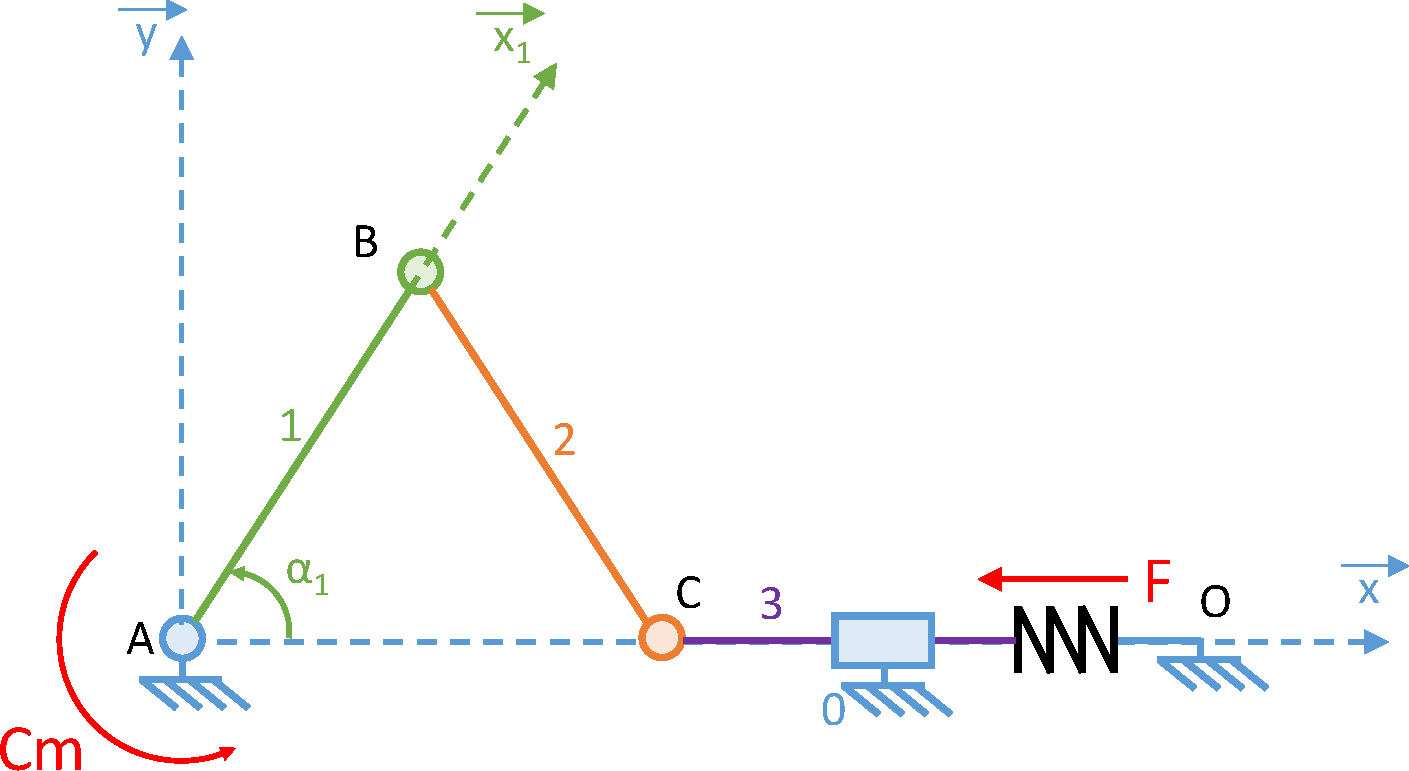
\includegraphics[width=0.95\linewidth]{img/schema-cin}
\end{center}
\end{minipage}\hfill
\begin{minipage}{0.45\linewidth}
Données:
\begin{itemize}
 \item $\overrightarrow{AB}=l.\overrightarrow{x_1}$,
 \item $\overrightarrow{AO}=L.\overrightarrow{x}$,
 \item $\alpha_1=(\overrightarrow{x},\overrightarrow{x_1})=(\overrightarrow{y},\overrightarrow{y_1})$,
 \item raideur du ressort: $k=100N.mm^{-1}$,
 \item $l=0.2m$,
 \item $L=0.2m$
\end{itemize}
\end{minipage}

~\ \vspace{1cm}

Comme le montre la figure, le couple du moteur est exercé sur la pièce $1$. L'action de la pièce $3$ sur le ressort a pour effet d'écraser ce dernier.

La position d'équilibre est difficile a déterminer car l'effort dans le ressort dépend de l'angle $\alpha_1$ qui est lié géométriquement à l'écrasement $x(t)$ du ressort.

L'objectif de cet exercice est de coder la résolution de cet exercice avec le lanage python.

L'étude se décomposera donc en deux parties, la première consiste a déterminer la valeur du coupe Cm en fonction de l'effort F. En ajoutant les lois caractérisant le comportement mécanique du ressort, un système d'équations sera obtenu. La partie seconde consistera à coder la résolution de ce système d'équations.

\paragraph{Question 1:} En isolant successivement les solides $1$, $2$ puis $3$. Déterminer la relation liant $F$ et $Cm$.

\paragraph{Question 2:} Donner la relation géométrique liant $x(t)$ et $\alpha_1$.

\paragraph{Question 3:} Donner l'équation mécanique liant $x(t)$ et $F$.

\paragraph{Question 4:} Proposer un code sous python permettant de résoudre ce système d'équations.

\end{document}
